\section{Assignment 7}

\subsection{Design the joint space inverse dynamics control law}

The goal is to implement the following architecture:

\begin{figure}[h]
\centering
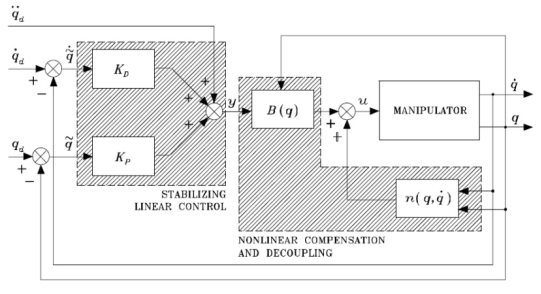
\includegraphics[keepaspectratio,width=0.4\textwidth]{inv_dyn_arch}
\caption{Joint space PD control law with gravity compensation architecture}
\end{figure}

The architecture works by linearizing non-linear dynamics and by decoupling each joint variable. It does so by implementing an inner feedback loop:

\begin{equation*}
\tau = B(q)y+n(q,\dot q)
\end{equation*}

where $n(q,\dot q) = C(q,\dot q)\dot q+g(q)$ and $y$ is controlled by the outer feedback loop:

\begin{equation*}
y = \ddot q_d+K_D(\dot q_d-q)+K_P(q_d-q)\;\;\;\;\text{with }K_P=50,K_D=10
\end{equation*}

The architecture was implemented in SIMULINK as follows:

\begin{figure}[h]
\centering
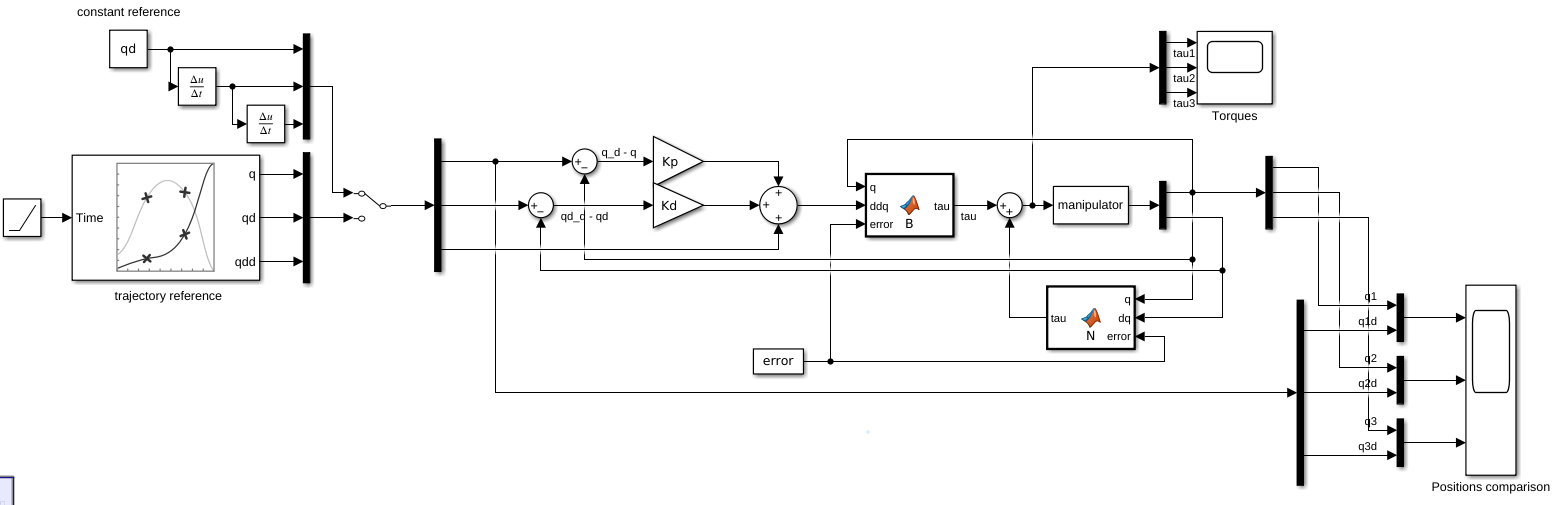
\includegraphics[keepaspectratio,width=0.8\textwidth]{inv_sim}
\caption{Joint space inverse control law SIMULINK model}
\end{figure}

The architecture is tested with a quintic polynomial trajectory that passes through the waypoints:

\begin{align*}
q_{d}\mid_{t=0.5} &= \begin{bmatrix}
\pi/3 & -0.2 & \pi/3
\end{bmatrix}\\
q_{d}\mid_{t=1} &= \begin{bmatrix}
-\pi/3 & -0.1 & \pi/4
\end{bmatrix}\\
q_{d}\mid_{t=1.5} &= \begin{bmatrix}
0 & -0.2 & 0
\end{bmatrix}\\
q_{d}\mid_{t=2} &= \begin{bmatrix}
\pi/2 & 0 & -\pi/4
\end{bmatrix}\\
q_{d}\mid_{t=2.5} &= \begin{bmatrix}
\pi/3 & -0.1 & \pi/4
\end{bmatrix}\\
q_{d}\mid_{t=3} &= \begin{bmatrix}
0 & 0 & 0
\end{bmatrix}
\end{align*}

The boundary conditions for the generation of the quintic trajectory are that the velocity and acceleration are null in each of the waypoints.

To show the effect of decoupling, the architecture was also tested against a constant reference $q_d=\begin{bmatrix}
\pi/1& -0.2&\pi
\end{bmatrix}$.

\begin{figure}[H]
\begin{minipage}{0.5\textwidth}
\centering
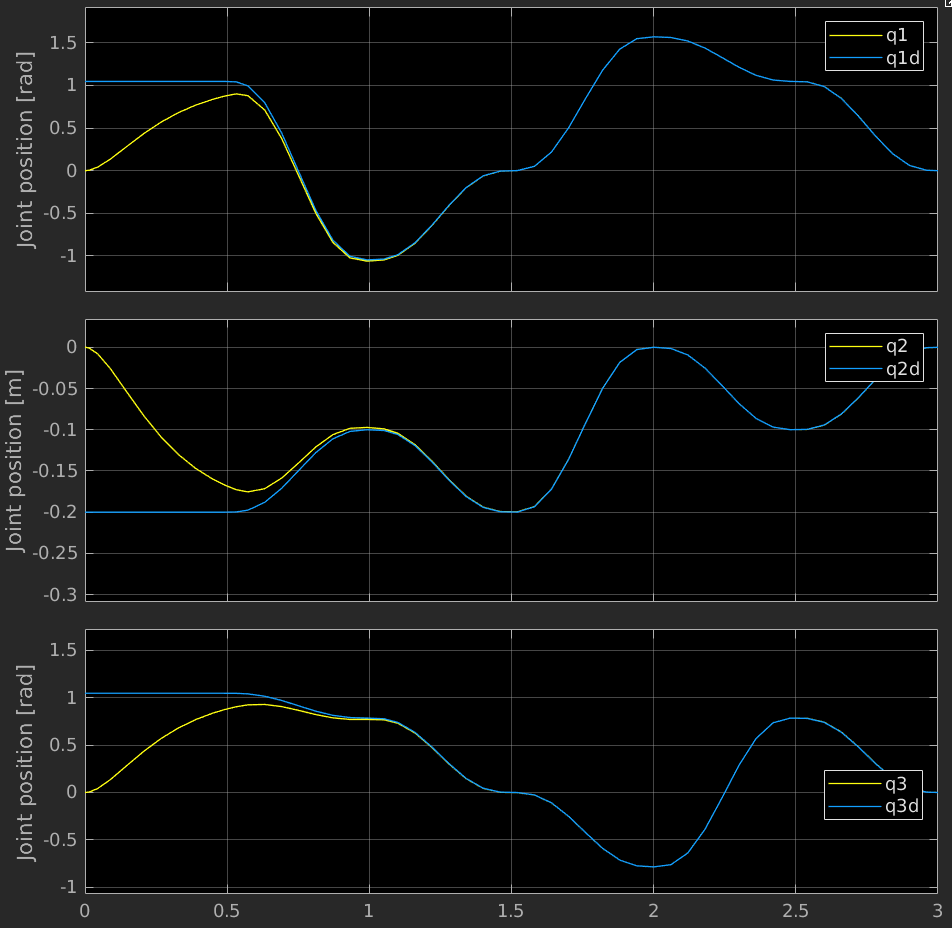
\includegraphics[keepaspectratio,width=\textwidth]{inv_correct}
\caption{Joint positions}
\end{minipage}
\begin{minipage}{0.5\textwidth}
\centering
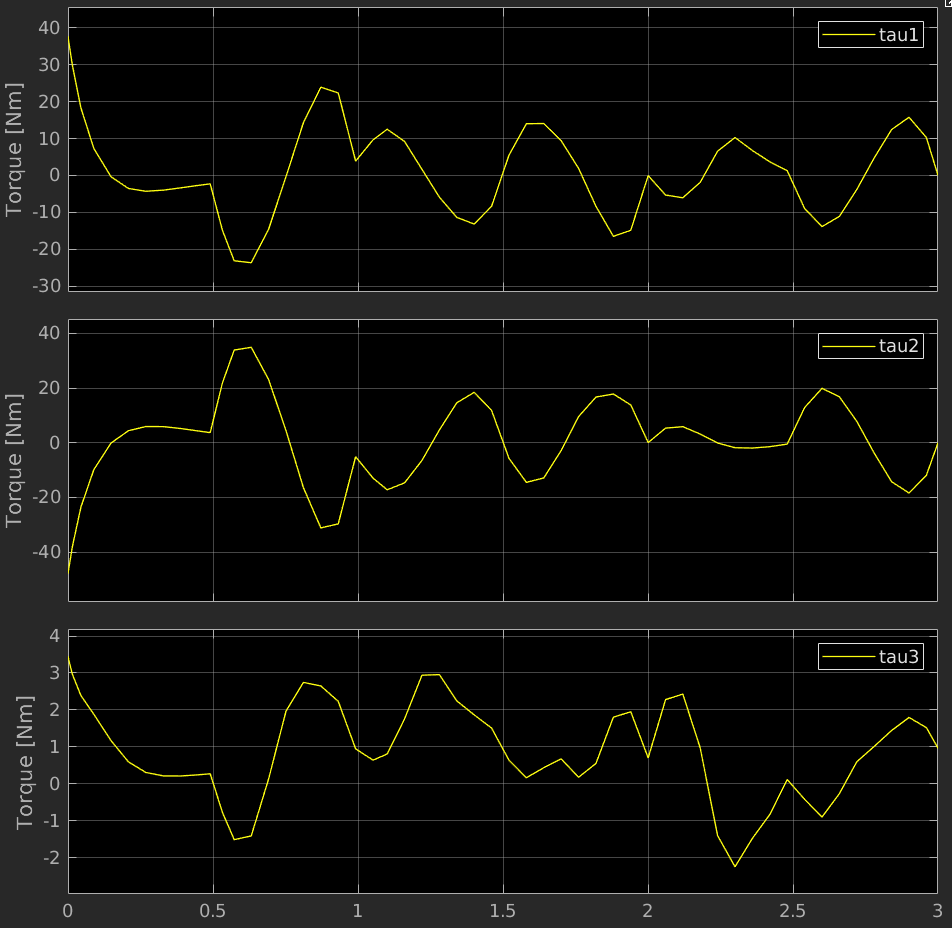
\includegraphics[keepaspectratio,width=\textwidth]{inv_correct_torque	}
\caption{Joint torques}
\end{minipage}
\end{figure}

\begin{figure}[H]
\centering
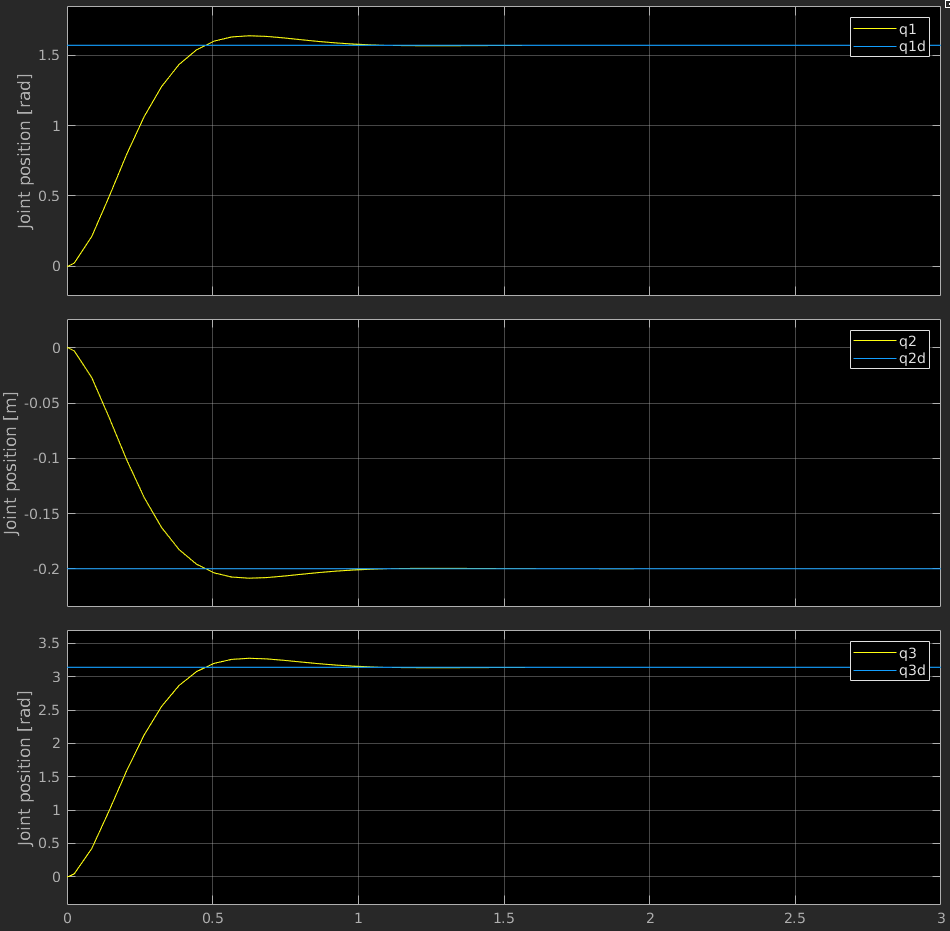
\includegraphics[keepaspectratio,width=0.65\textwidth]{inv_same_beh}
\caption{Joint positions - constant reference, decoupling}
\end{figure}

\subsection{Check the behaviour of the control law when the B, C and g values are different than the true ones}

\begin{figure}[H]
\centering
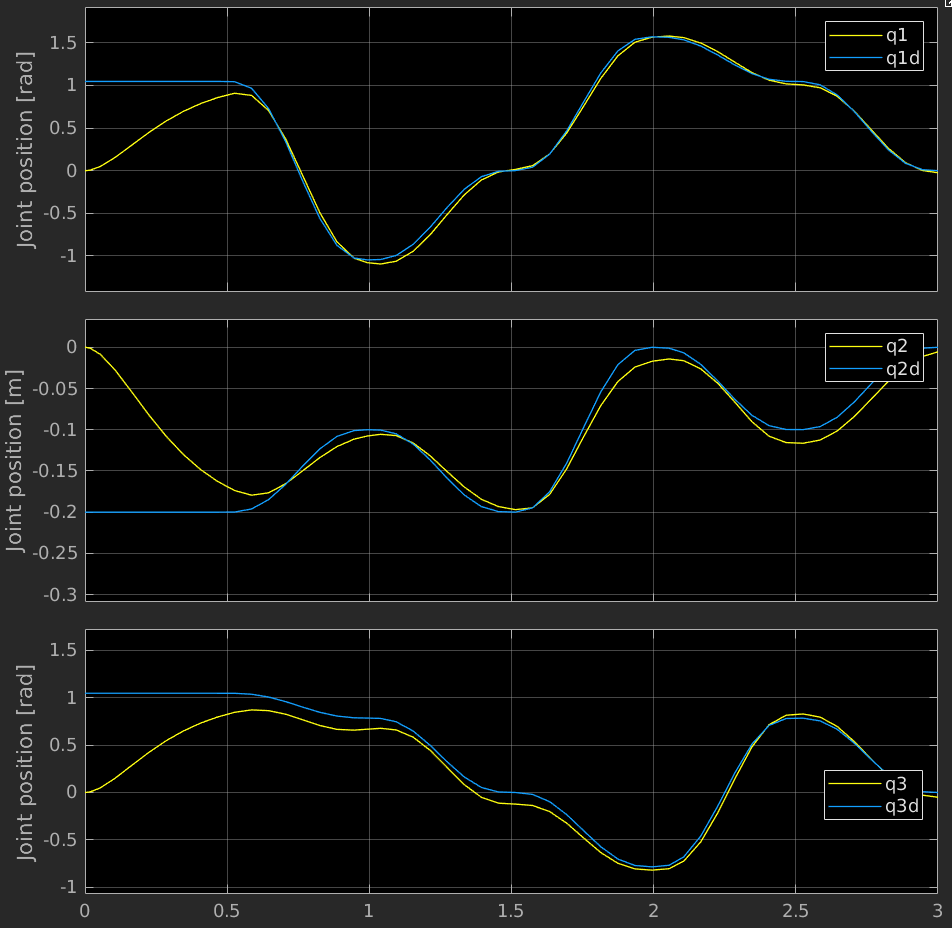
\includegraphics[keepaspectratio,width=0.65\textwidth]{inv_wrongB}
\caption{Joint positions - changed values of the link masses}
\end{figure}

\subsection{What happens to the torque values when the settling time of the equivalent second order systems is chosen very small?}

\begin{figure}[H]
\centering
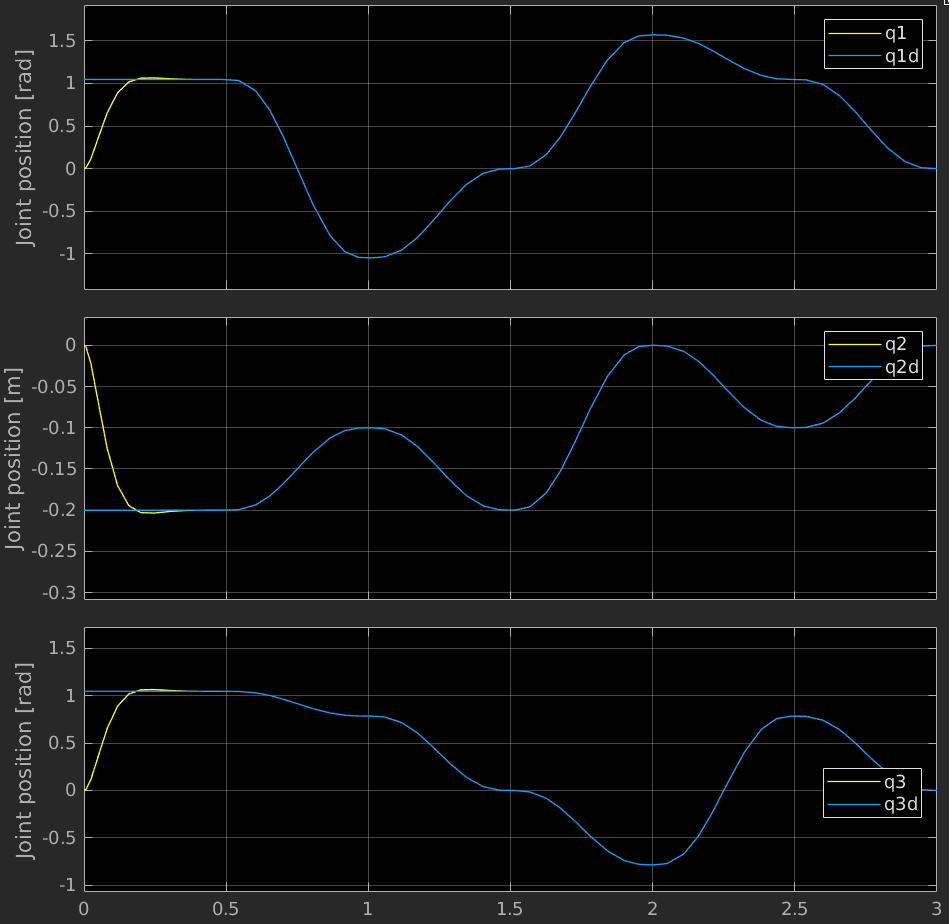
\includegraphics[keepaspectratio,width=0.6\textwidth]{inv_small_rising}
\caption{Joint positions - $K_P=500,K_D=35$}
\end{figure}
\begin{figure}[H]
\centering
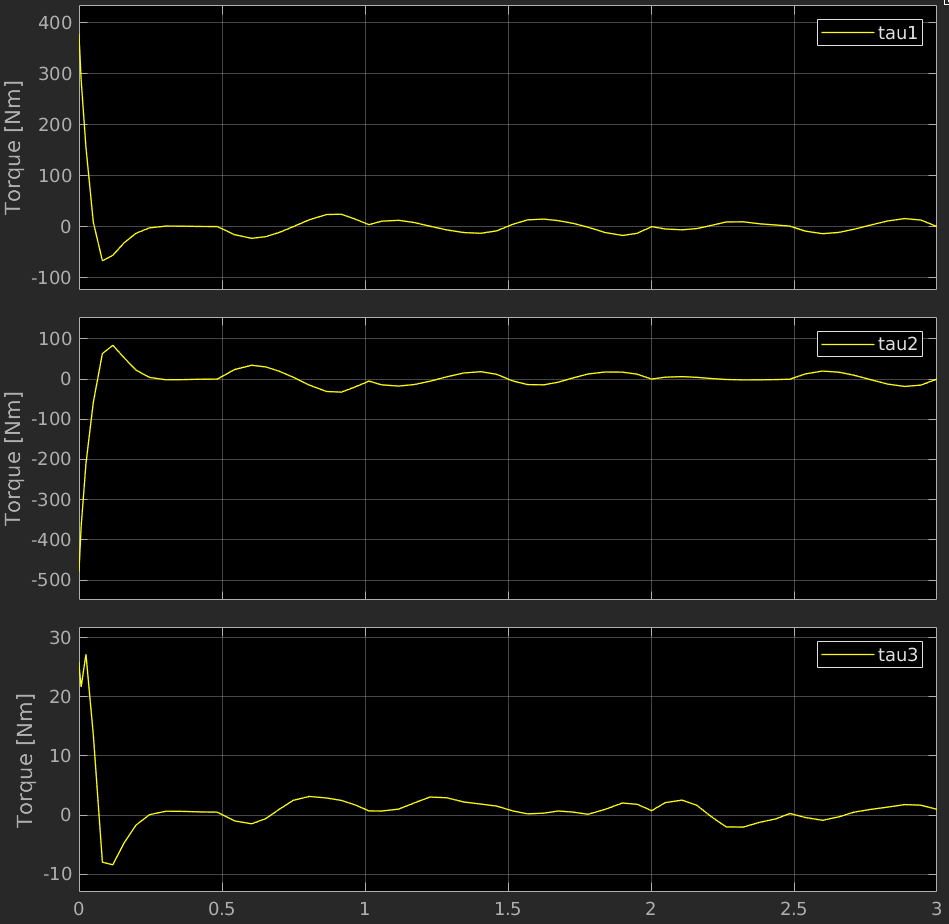
\includegraphics[keepaspectratio,width=0.6\textwidth]{inv_small_rising_torque}
\caption{Joint torques - $K_P=500,K_D=35$}
\end{figure}